\chapter{Induction heating of a graphite crucible}

\modinfo{Directory}{InductionHeating}
\modinfo{Solvers}{\Idx{StatMagSolve}}
\modinfo{Tools}{\Idx{ElmerGrid}, editor}
\modinfo{Dimensions}{2D, Axi-Symmetric}

\subsection*{Case definition}

At high temperatures the most practical 
method to heat up the crucible 
is by electromagnetic induction. 
The induction coil generates an alternating 
current that flows through the crucible. 
The Ohmic resistance encountered by this current dissipates 
energy, thereby directly
heating the crucible via internal heat generation.

The tutorial case is a simple axi-symmetric crucible that could be
used, for example, to grow silicon carbide (SiC) by the sublimation method.
The crucible 
is made of dense graphite and isolated by 
porous graphite. At the bottom of the crucible there is
some SiC powder. The physical properties of the 
material are given in Table~\ref{tab:ind_heat1}. The dimensions of the
induction heating crucible are given in Table~\ref{tab:ind_heat2}.
Additionally, the powder thickness is 1.0~cm and there are 10 spirals
in the coil.
The frequency of induction heating $f$ is 50 kHz and the current 
$I$ is 10 A.
The permeability of the space is $4\pi 10^{-7}$
if the other variables are in SI-units.

\begin{table}
\caption{Material parameters of the crucible}
\label{tab:ind_heat1}
\begin{center}
\begin{tabular}{llll} \hline
material & $\varepsilon$  & $\kappa$ [W/mk] & $\sigma$ (1/$\Omega$m) \\ \hline 
graphite  &      0.7   &          10.0  &          2.0E4 \\
insulation &      0.9   &          1.0   &          2.0E3  \\
powder    &      0.5   &          25.0  &          1.0E4 \\ \hline
\end{tabular}
\end{center}
\end{table}

\begin{table}
\caption{Dimensions of the crucible}
\label{tab:ind_heat2}
\begin{center}
\begin{tabular}{lllll} \hline
body part &  $r_{inner}$ & $r_{outer}$ & $h_{inner}$ & $h_{outer}$ \\ \hline
graphite  &  2.0   &  2.5 & 6.0 & 8.0 \\
insulation &  2.5   &  4.0 & 8.0 & 12.0 \\
coil      &  5.0   & 5.5  &     & 8.0  \\ \hline
\end{tabular}
\end{center}
\end{table}


\subsection*{Solution Procedure}

At low frequencies the free charges may be neglected and the 
induction heating problem may be solved in terms 
of an magnetic vector potential. The proper solver to do
this is \texttt{StatMagSolver}.
However, the induction heating problem can only be modeled if the helicity 
of the coil is neglected and an average current density is assumed.
This current density may be computed easily when the 
area of the coil is known $j_0=n I / A$, where $A$ is the 
coil area.

The mesh for this problem may easily be created by ElmerGrid.
The provided mesh is quite sufficient for this case
but for higher frequencies the mesh should be tuned 
to solve the thin boundary layers.
The computational mesh is created from file \texttt{crucible.grd} by the 
command 
\ttbegin
ElmerGrid 1 2 crucible
\ttend

The mesh consists of 5 different bodies which need 4
different materials sets. Only on set of boundary conditions 
are required for the external boundary. Thus the header 
information of the command file is as follows
\ttbegin
Header
  Mesh DB "." "crucible"
  Include Path ""
  Results Directory ""
End
\ttend
%
In the \texttt{Simulation} section the coordinate system and
time dependency is set, among other things. Also we know that
the equation is linear and therefore only one steady state
iteration is requited. If the electric properties depend on 
the magnitude of the field several iterations are required.
\ttbegin
Simulation
  Coordinate System = "Axi Symmetric"
  Simulation Type = Steady State
  Steady State Max Iterations = 1
  Output File = "crucible.result"
  Post File = "crucible.vtu"
End
\ttend
%
In the \texttt{Constants} section the permittivity of 
vacuum must be given.
\ttbegin
Constants
  Permittivity Of Vacuum = 8.8542e-12
End
\ttend
%
In the differential equation for the magnetic vector potential the 
source the is the current density. Thus, it is given in the
\texttt{Body Force} section. 
\ttbegin
Body Force 1
  Current Density = 2.5e5
End
\ttend
%
In the \texttt{Body} section the different bodies are assigned 
with correct equation sets and material parameters, for example
\ttbegin
Body 3
  Name = "Insulation"
  Equation = 1
  Material = 2
End
\ttend
%
In the \texttt{Equation} block all the relevant solvers are 
set to active.
\ttbegin
Equation
  Name = "Vector Potential Equation"
  Active Solvers = 1
End
\ttend
%
The only solver in this simple tutorial is the solver for the magnetic
vector potential. Look for the relevant model manual for information
about the options. Here the equation is solved iteratively and the
local Joule heating and magnetic flux are computed as a postprocessing
step. The Joule heating is scaled so that the total heating power is
3.0~kW. This option may be used when the total heating efficiency is
known.  The nonlinear solver parameters are not really needed as the
material parameters are constant. Sometimes the parameters may depend
on the magnetic field and thus the nonlinear problem must be solved
iteratively.
%
\ttbegin
Solver 1
  Equation = Potential Solver
  Variable = Potential
  Variable DOFs = 2

  Angular Frequency = Real 50.0e3
  Calculate Joule Heating = Logical True
  Calculate Magnetic Flux = Logical True
  Desired Heating = Real 3.0e3

  Procedure = "StatMagSolve" "StatMagSolver"
  Linear System Solver = Iterative
  Linear System Iterative Method = BiCGStab
  Linear System Max Iterations = 300
  Linear System Convergence Tolerance = 1.0e-10
  Linear System Preconditioning = ILU1
  Linear System ILUT Tolerance = 1.0e-03
  Linear System Residual Output = 1
  Nonlinear System Max Iterations = 1
  Nonlinear System Convergence Tolerance = 1.0e-6
  Nonlinear System Relaxation Factor = 1
  Steady State Convergence Tolerance = 1.0e-6
End
\ttend
%
In the \texttt{Material} sections all the necessary 
material parameters are given, for example
\ttbegin
Material 2
  Name = "Insulation"
  Electric Conductivity = 2.0E3
End
\ttend
%
The magnetic field must vanish at infinity. Unfortunately the
computational domain is bounded and therefore the infinite
distance becomes very finite. A proper distance may be checked
by gradually increasing it until no change in the result occurs.
%
\ttbegin
Boundary Condition 1
  Target Boundaries = 1
  Potential 1 = Real 0.0
  Potential 2 = Real 0.0
End
\ttend

\subsection*{Results}

With the given computational mesh the problem is solved in 
a few seconds. With the 20\,072 bilinear elements the heating
efficiency is $16.9$ W. The corresponding results are shown
in Fig.~\ref{fig:ind_heat1}.

\begin{figure}
\begin{center}
  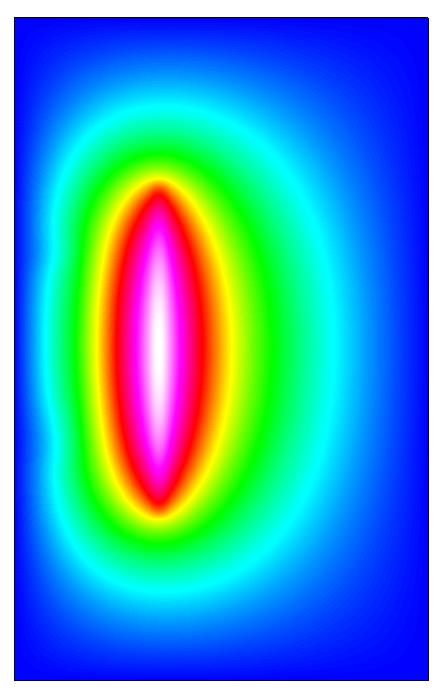
\includegraphics[height=0.4\textwidth]{induct2}
  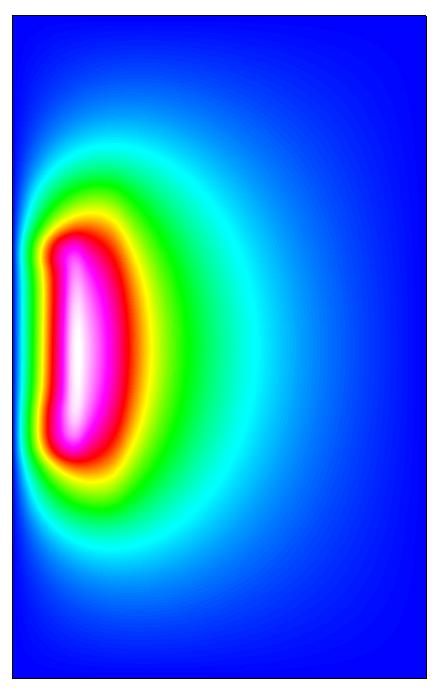
\includegraphics[height=0.4\textwidth]{induct3}
  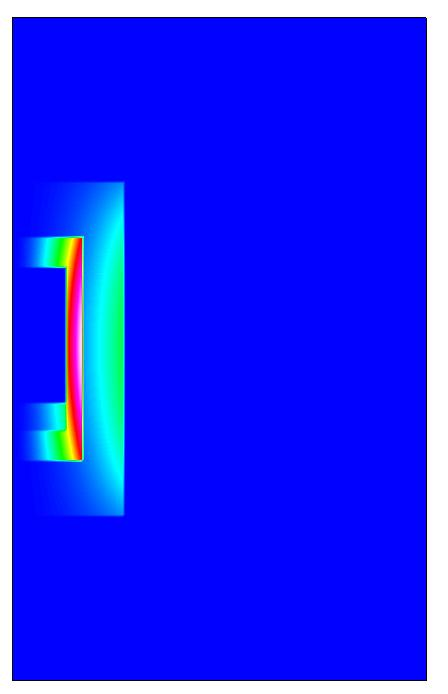
\includegraphics[height=0.4\textwidth]{induct1}
\end{center}
\caption{Induction heating of a simple crucible. 
a) in-phase component of the vector potential
b) out-of-phase component of the vector potential
c) Joule losses in the conductors}
\label{fig:ind_heat1}
\end{figure}

